% Straight up stealing preamble from Eli Holmes 
%%%%%%%%%%%%%%%%%%%%%%%%%%%%%%%%%%%%%%START PREAMBLE THAT IS THE SAME FOR ALL EXAMPLES
\documentclass{article}

%Required: You must have these
\usepackage{Sweave}
\usepackage{graphicx}
\usepackage{tabularx}
\usepackage{hyperref}
\usepackage{natbib}
\usepackage{pdflscape}
\usepackage{array}
\usepackage{gensymb}
\usepackage{authblk}
\renewcommand{\baselinestretch}{1.8}
%\usepackage{lineno}
%\usepackage[backend=bibtex]{biblatex}
%Strongly recommended
 %put your figures in one place
 
%you'll want these for pretty captioning
\usepackage[small]{caption}

\setkeys{Gin}{width=0.8\textwidth} %make the figs 50 perc textwidth
\setlength{\captionmargin}{30pt}
\setlength{\abovecaptionskip}{0pt}
\setlength{\belowcaptionskip}{10pt}
% manual for caption http://www.dd.chalmers.se/latex/Docs/PDF/caption.pdf

%Optional: I like to muck with my margins and spacing in ways that LaTeX frowns on
%Here's how to do that
 \topmargin -2cm 
 \oddsidemargin -0.04cm 
 \evensidemargin -0.04cm % same as oddsidemargin but for left-hand pages
 \textwidth 16.59cm
 \textheight 22.94cm 
 %\pagestyle{empty} % Uncomment if don't want page numbers
 \parskip 7.2pt  % sets spacing between paragraphs
 %\renewcommand{\baselinestretch}{1.5} 	% Uncomment for 1.5 spacing between lines
\parindent 0pt% sets leading space for paragraphs
\usepackage{setspace}
%\doublespacing

%Optional: I like fancy headers
\usepackage{fancyhdr}
\pagestyle{fancy}
\fancyhead[LO]{Experimental climate change}
\fancyhead[RO]{2018}

%%%%%%%%%%%%%%%%%%%%%%%%%%%%%%%%%%%%%%END PREAMBLE THAT IS THE SAME FOR ALL EXAMPLES

%Start of the document
\begin{document}

% \SweaveOpts{concordance=TRUE}
\bibliographystyle{/Users/aileneettinger/citations/Bibtex/styles/ecol_let.bst}

\title{How does soil moisture interact with temperature to affect phenology?}
\author[1,2,a]{A.K. Ettinger}
\author[3,b]{J.S. Dukes}
\author[4,c]{M.R. Johnston}
\author[5,d]{C.R. Rollinson}
\author[1,4,6,e]{E.M. Wolkovich}

% ESA authors: Ailene K. Ettinger, Jeffrey S. Dukes, Miriam R. Johnston, Christy R.  Rollinson, and Elizabeth M. Wolkovich.
%\author[3,b]{I. Chuine}

%\author[4,5,c]{B.I. Cook}


%\author[7,e]{A.M. Ellison}

%\author[9,g]{A.M. Panetta}
%\author[11,12,i]{Y. Vitasse}

\affil[1]{Arnold Arboretum of Harvard University, Boston, Massachusetts 02131, USA}

\affil[2]{Tufts University, Medford, Massachusetts 02155, USA}

%\affil[3]{CEFE UMR 5175, CNRS, Universit\'e de Montpellier,Universit\'e Paul-Val\'ery Montpellier, EPHE IRD, Montpellier, France}

%\affil[4]{Lamont-Doherty Earth Observatory, Columbia University, Palisades, New York 10964, USA}

%\affil[5]{NASA Goddard Institute for Space Studies, New York, New York 10025, USA}

\affil[3]{Department of Forestry \& Natural Resources and Department of Biological Sciences, Purdue University, West Lafayette, Indiana 47907, USA}

%\affil[7]{Harvard Forest, Harvard University, Petersham, Massachusetts 01366, USA}

\affil[4]{Department of Organismic \& Evolutionary Biology, Harvard University, Cambridge, Massachusetts 02138, USA}

%\affil[9]{Department of Ecology and Evolutionary Biology, University of Colorado, Boulder, Colorado 80309, USA}

\affil[5]{The Morton Arboretum, Lisle, Illinois 60532, USA}

%\affil[11]{Institute of Geography, University of Neuch\^atel, Neuch\^atel, Switzerland}

%\affil[12]{Swiss Federal Institute for Forest, Snow and Landscape Research WSL, Neuch\^atel, Switzerland}

\affil[6]{Forest \& Conservation Sciences, Faculty of Forestry, University of British Columbia, Vancouver, BC, Canada}

\affil[a]{Corresponding author; email: aettinger@fas.harvard.edu; phone: 781-296-4821; mailing address: 1300 Centre Street, Boston, Massachusetts 02140, USA }

%\affil[b]{isabelle.chuine@cefe.cnrs.fr}

%\affil[c]{bc9z@ldeo.columbia.edu}

%\affil[d]{jsdukes@purdue.edu}

%\affil[e]{aellison@fas.harvard.edu}

%\affil[f]{mjohnston@g.harvard.edu}

%\affil[g]{anne.panetta@colorado.edu}

%\affil[h]{crollinson@mortonarb.org}

%\affil[i]{yann.vitasse@wsl.ch}

%\affil[j]{e.wolkovich@ubc.ca}


\date{\today}
\maketitle %put the fancy title on
%\tableofcontents %add a table of contents

\textbf{Statement of authorship} 
All authors conceived of this manuscript, which began at a Radcliffe Exploratory Seminar in 2016, and all authors contributed to manuscript revisions. AKE and EMW conceived of the idea for the literature review, database compilation, and related Radcliffe Exploratory Seminar. AKE compiled the datasets; AKE analyzed the data and created the figures; AKE wrote the manuscript.

\textbf{Data Accessibility} %Data accessibility statement: The statement must confirm that, should the manuscript be accepted, the data supporting the results will be archived in an appropriate public repository such as Dryad or Figshare and the data DOI will be included at the end of the article.
The MC3E and ExPhen databases are available at KNB \citep{ettinger2018}, along with all R code from the analyses included in this paper. (Currently, metadata are published there; the full databases and R code are available to reviewers on github.) 

\textbf{Running title} 
\textbf{Key words} global warming, warming experiment, microclimate, soil moisture, phenology, budburst, direct and indirect effects, active-warming, target temperature


\clearpage
%%%%%%%%%%%%%%%%%%%%%%%%%%%%%%%%%%%%%%%%%%%%%%%%%%%
%\linenumbers

\section*{Outline}
\begin{enumerate}
\item{How do climate manipulations affect soil moisture and temperature?}
\item{Approach: Use MC3E database. Fit multilevel models of soil moisture as a function of temperature and precipitation treatments.}
\noindent For this we need two equations where we evaluate the effects of experimenal temperature (\textit{eT}) and experimental preciptation (\textit{eP}) treatments on soil moisture and temperature. We're hoping to nest year within site on the intercept and slopes:
\begin{equation}
y_{i}=\alpha_{site[year[doy[i]]]}+ \beta_{1 site[i]}eT_i+\beta_{2 site[i]}eP_i+\beta_{3 site[i]}eT_ieP_i+\epsilon_{i}
\end{equation}
\begin{equation}
\alpha_{site[year[doy]]}\sim N(\mu_{site[year]}, \sigma_{site[year]})
\end{equation}

\begin{equation}
\mu_{site[year]} \sim N(\mu_{sy}, \sigma_{sy})
\end{equation}

\begin{equation}
\mu_{sy} \sim N(\mu_{s}, \sigma_{s})
\end{equation}

\begin{equation}
\beta_{1 site} \sim N(\mu_{\beta1}, \sigma_{\beta1})
\end{equation}

\begin{equation}
\beta_{2 site} \sim N(\mu_{\beta2}, \sigma_{\beta2})
\end{equation}

\begin{equation}
\beta_{3 site} \sim N(\mu_{\beta3}, \sigma_{\beta3})
\end{equation}

\begin{equation}
\beta_{1 sp} \sim N(\mu_{\beta1}, \sigma_{\beta1})
\end{equation}

\begin{equation}
\beta_{2 sp} \sim N(\mu_{\beta2}, \sigma_{\beta2})
\end{equation}

\begin{equation}
\beta_{3 sp} \sim N(\mu_{\beta3}, \sigma_{\beta3})
\end{equation}

\item{Does warming affect soil moisture similarly to warming in experimental and non-experimental data?}

\par Compile data from Duke Forest (maybe just soil moisture?) and from Harvard Forest (soil moisture and O'Keefe phenology data). Think on best model and how to model temperature as \textit{y} variable ... here's one idea where \textit{y} could be daily moisture data across multiple years and \textit{T} would be MAT and \textit{P} would be percent different than mean for that year:



\begin{equation}
y_{i}=\alpha_{doy[i]}+\beta_{1 site[i]}T_i+\beta_{2 site[i]}P_i+\beta_{3 site[i]}T_iP_i+\epsilon_{i}
\end{equation}

\begin{equation}
\alpha_{doy} \sim N(\mu_{doy}, \sigma_{doy})
\end{equation}
\noindent First we need to use seasonal or annual temperature (\textit{T}) and soil moisture (\textit{S}) data to predict phenology (so here textit{y} is DOY):

\begin{equation}
y_{i}=\alpha_{site[year[i]]}+ \alpha_{sp[i]}+\beta_{1 sp[i]}T_i+\beta_{2 sp[i]}S_i+\beta_{3 sp[i]}T_iS_i+\epsilon_{i}
\end{equation}

\begin{equation}
\alpha_{site[year]} \sim N(\mu_{sy}, \sigma_{sy})
\end{equation}

\begin{equation}
\mu_{sy} \sim N(\mu_{s}, \sigma_{s})
\end{equation}

\begin{equation}
\alpha_{sp} \sim N(\mu_{sp}, \sigma_{sp})
\end{equation}


\item{How does soil moisture affect phenology? How does soil moisture affect GDDcrit?}
\begin{enumerate}
\item{Compile phenology data that goes with climate data in MC3E database. (Name the phenology database!)}
\item{Fit models with soil moisture, temperature, and interaction to phenology data (budburst, leafout, flowering, fruiting, senesence? (See what phenophases have enough data.)}
\end{enumerate}
\noindent Does the effect of soil moisture on phenology differ between experiments and observational data? We can then combine equations from Question 1 (which predict MAT and soil moisture on an annual scale, we hope) with equations from Questions 3 (at the annual scale) to answer: how much does 1 degree change in target temperature (\textit{eT}) affect phenology, if this were the only effect of the experiment? Similarly, how much does 50\% change in precipitation (\textit{eP}) affect phenology, if this were the only effect of the experiment? And how big a change does each make acknowledging that they both change moisture and temperature together? We can do this by plugging in different values of \textit{eT} (e.g., all 1 C, then try with all 2 C) and \textit{eP} to calculate different outcomes of moisture and temperature which we can evaluate in the equations in Question 3 to assess changes in phenology.
\end{enumerate}
%\section*{Abstract}

%\section* {Introduction}

%\section* {Methods}

%\section* {Results}
%\section* {Discussion}

%\section* {Conclusions}

\bibliography{/Users/aileneettinger/citations/Bibtex/mylibrary}
\clearpage
\section* {Figures}
\clearpage
 \begin{figure}[h]
\centering
 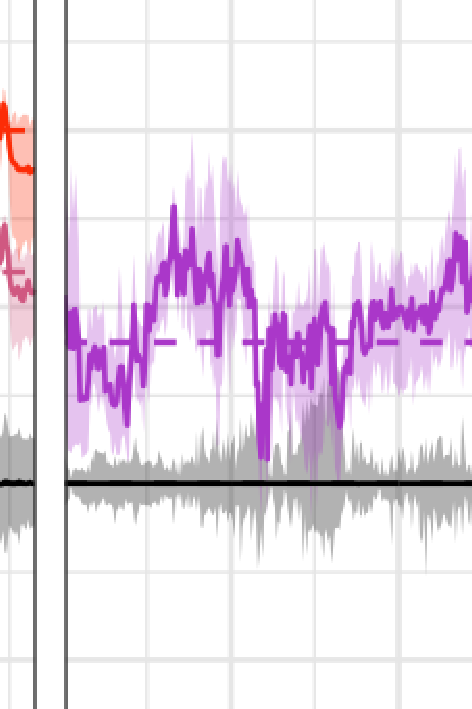
\includegraphics{/Users/aileneettinger/git/radcliffe/Analyses/figures/WarmingEffects_TimeSeries_SoilTemp1Mean_Deviation_NoPrecip.png}
 \caption{\textbf{Deviations in daily observed warming from mean control soil temperature for 12 study sites,} excluding data from plots that manipulated precipitation. We show soil, rather than above-ground, temperature, as this was the most frequently recorded temperature variable in the MC3E database. Solid lines show observed difference between warming treatment (colors) and control (black) plots, averaged across replicates and years; shading shows 95\% confidence intervals. Dashed lines represent target warming levels. (Note that the following studies had no explicit target temperature: exp06, exp11, exp12; for these studies, we used their reported level of warming.) Two sites not shown here did not monitor soil temperature. Experimental sites are ordered by low to high mean annual soil temperature (shown in the upper right corner of each panel). The heating type is listed in parentheses next to the site number (IR= infrared, soil= soil cables, air= forced air).} %The number of temperature treatment levels vary from one (e.g. exp08, exp11) to nine (exp07 and exp10, which used an unreplicated regression design). Daily temperature values were obtained by averaging across years for each day of the year in each temperature treatment in each study. 
 \label{fig:effwarm}
 \end{figure}

%%%%%%%%%%%%%%%%%%%%%%%%%%%%%%%%%%%%%%%%
\end{document}
%%%%%%%%%%%%%%%%%%%%%%%%%%%%%%%%%%%%%%%%
